In this task we are aim to find the value of the option, $V(S,t)$ as a function of the underlying asset price $S$ at $t=0$, i.e., $V(S,t=0)$. In order to so, we are given two pairs of specific parameters, 
\begin{enumerate}[wide, labelindent=0cm]
	\item $\beta=1$ and $\sigma = 0.381$, and all other parameters as standard.
	\item $\beta=0 0.808$ and $\sigma=0.66$, and all other parameters as standard.
\end{enumerate}

\begin{figure}[htbp]
	\centering
	\captionsetup{width=.5\linewidth}
	\begin{subfigure}[b]{0.49\textwidth}
		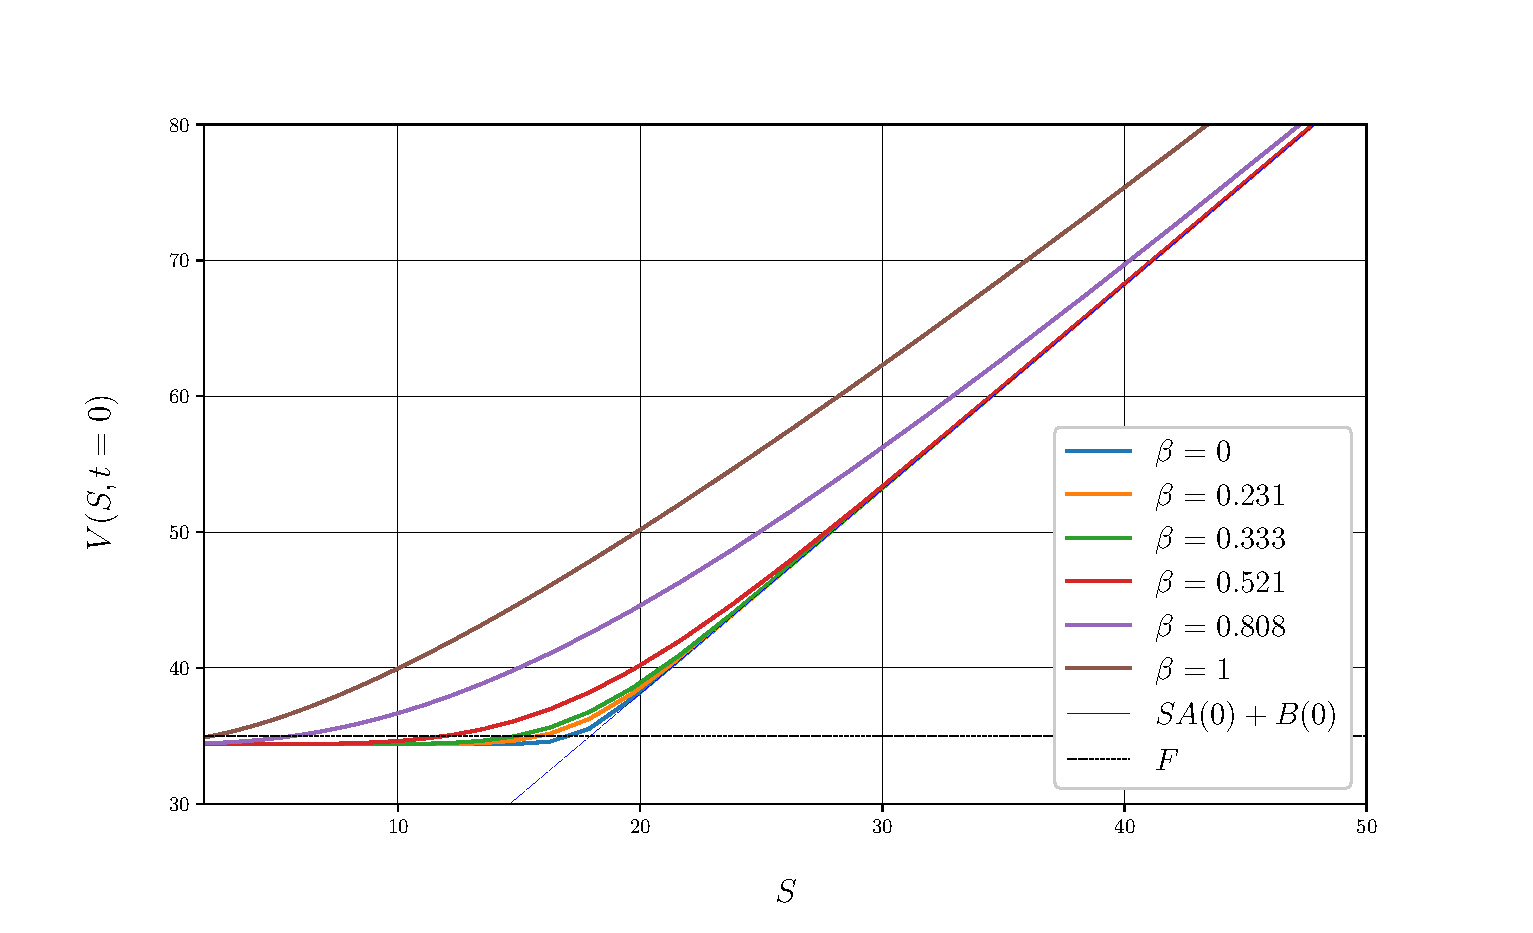
\includegraphics[width=\textwidth]{img/Q1/ComparisonDifferentBetas_sigma06600.eps}
		\captionsetup{width=.8\linewidth}
		\caption{Value of the option for different $\beta$ as $S$ becomes larger with $\sigma = 0.381$.}
		\label{changingBeta}
	\end{subfigure}
	\begin{subfigure}[b]{0.49\textwidth}
		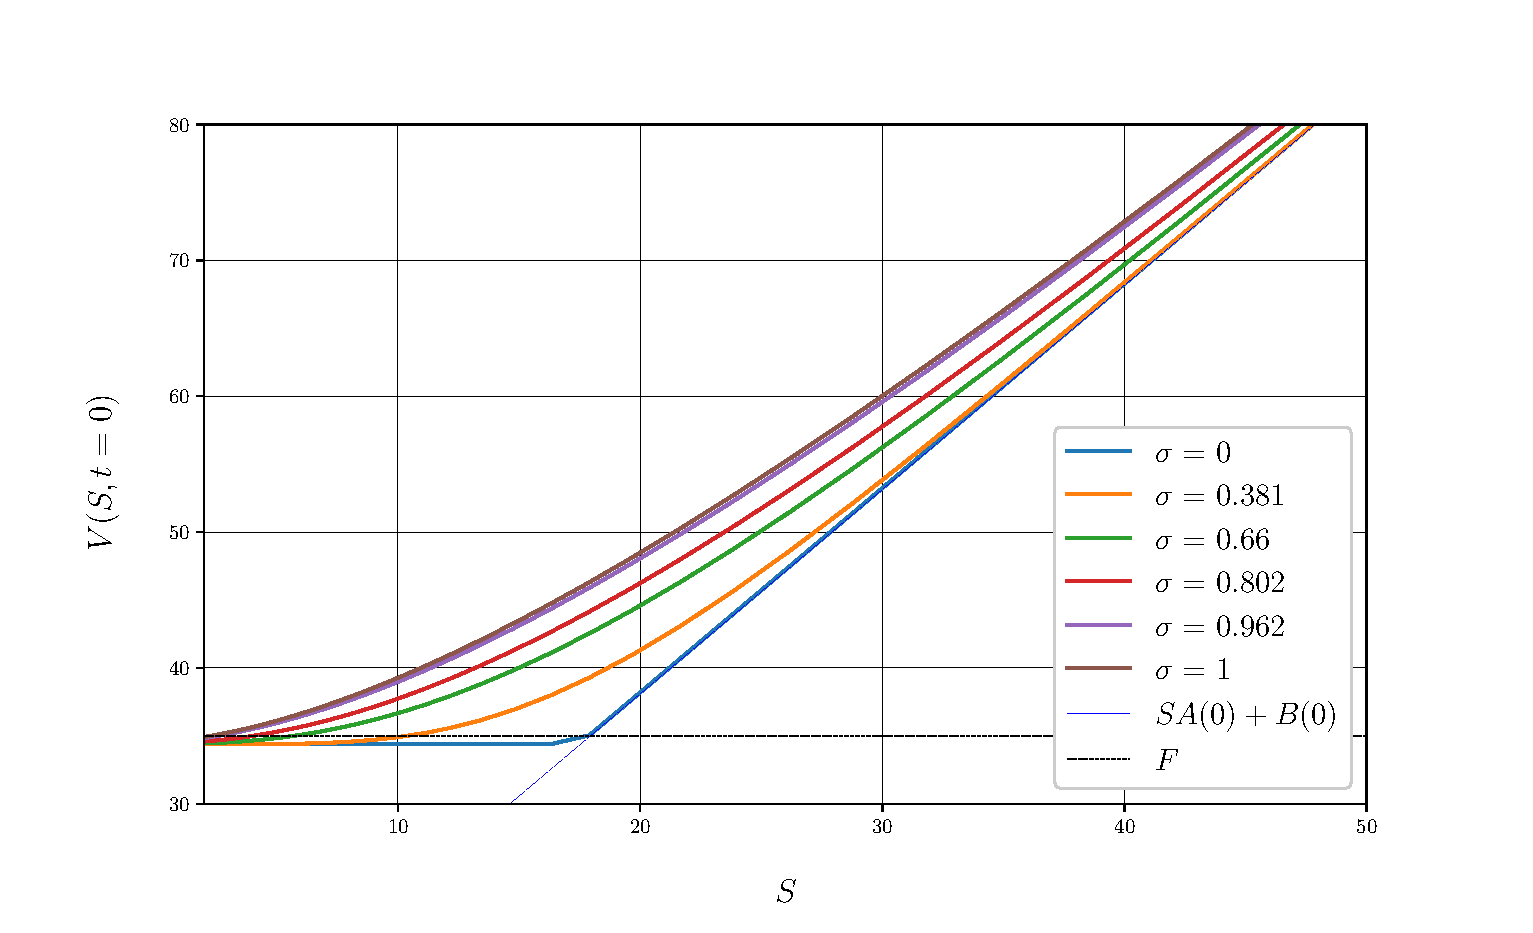
\includegraphics[width=\textwidth]{img/Q1/ComparisonDifferentSigmas_beta0808.eps}
		\captionsetup{width=.8\linewidth}
		\caption{Value of the option for different $\sigma$ as $S$ becomes larger with $\beta=0.808$.}
		\label{changingSigma}
	\end{subfigure}
	\caption{Value of the option as $S$ becomes larger for different parameters.}
	\label{S_larger}
\end{figure}

The idea is to see what happen when $\beta$ and $\sigma$ are changed.

On the one hand, both $\beta$  and $\sigma$ contributes to the term 
\begin{equation}
	\frac{1}{2}\sigma^2S^{2\beta}\partial_S^2 V.
\end{equation}

Note from (\ref{general_pde}) that
\begin{equation}
	V = \frac{1}{r}\left(\partial_t V + \frac{1}{2}\sigma^2 S^{2\beta}\partial_{SS} V + \kappa\left(\theta(t) - S\right)\partial_S + Ce^{-\alpha t}\right);
\end{equation}
which means that, when all of the parameters are the same but not $\beta$ and $\sigma$, then we can understand $V(S,t)$ as
\begin{equation}\label{useful}
	V = \frac{1}{2r}\sigma^2 S^{2\beta}\partial_{SS} V + \text{other}.
\end{equation}

On the other hand, we now that when $S$ becomes larger, $V(S,t)$ tends to $S A(t) + B(t)$, so the contribution of $\beta$ and $\sigma$ is significant when $S$ is somehow small. Moreover, it is obvious from (\ref{useful}) that $V$ becomes smaller as $\sigma$ and $\beta$ becomes smaller. Particularly, when $\beta \to 0$, then
\begin{equation}
	V \to  \frac{1}{2r}\sigma^2 S^{2}\partial_{SS} V + \text{other};
\end{equation}
and, when $\sigma\to 0$, 
\begin{equation}
	V \to  \text{other},
\end{equation}
and the contribution of the second derivative with respect of $S$ is null, i.e., it's linear on $S$ (tending to $F$ for small $S$). This is coherent with Figure \ref{S_larger}, in which we can see how the value of the option flattens before the cross of $F$ and $S A(0) + B(0)$, i.e., when
\begin{equation}
	S^* = \frac{F-B(0)}{A(0)} = 17.94670.
\end{equation} 

This means that when $S < S^*$, then $V(S,0) \to F$ as $\sigma, \beta\to0$. Intuitively speaking, $\sigma$ is the volatility of the process, so the larger the sigma, the larger the random fluctuation from the Brownian Motion. In some sense, it increases the randomness of the stock price. On the other hand, $\beta$ is the elasticity of the stock price, meaning that $\sigma S^\beta$ is the instantaneous volatility of the stock price, i.e., 
\begin{equation}
	\frac{\partial_S \left(\sigma S^\beta\right)}{\sigma S^{\beta}/S} =\frac{\sigma \beta S^{\beta-1}}{\sigma S^{\beta-1}} = \beta,
\end{equation}
which means that it is the percentange of change in instantaneous volatility as $S$ changes. If $\beta < 1$, then the volatility increases as the stock price decreases, and viceversa.
\begin{figure}[htbp]
	\centering
	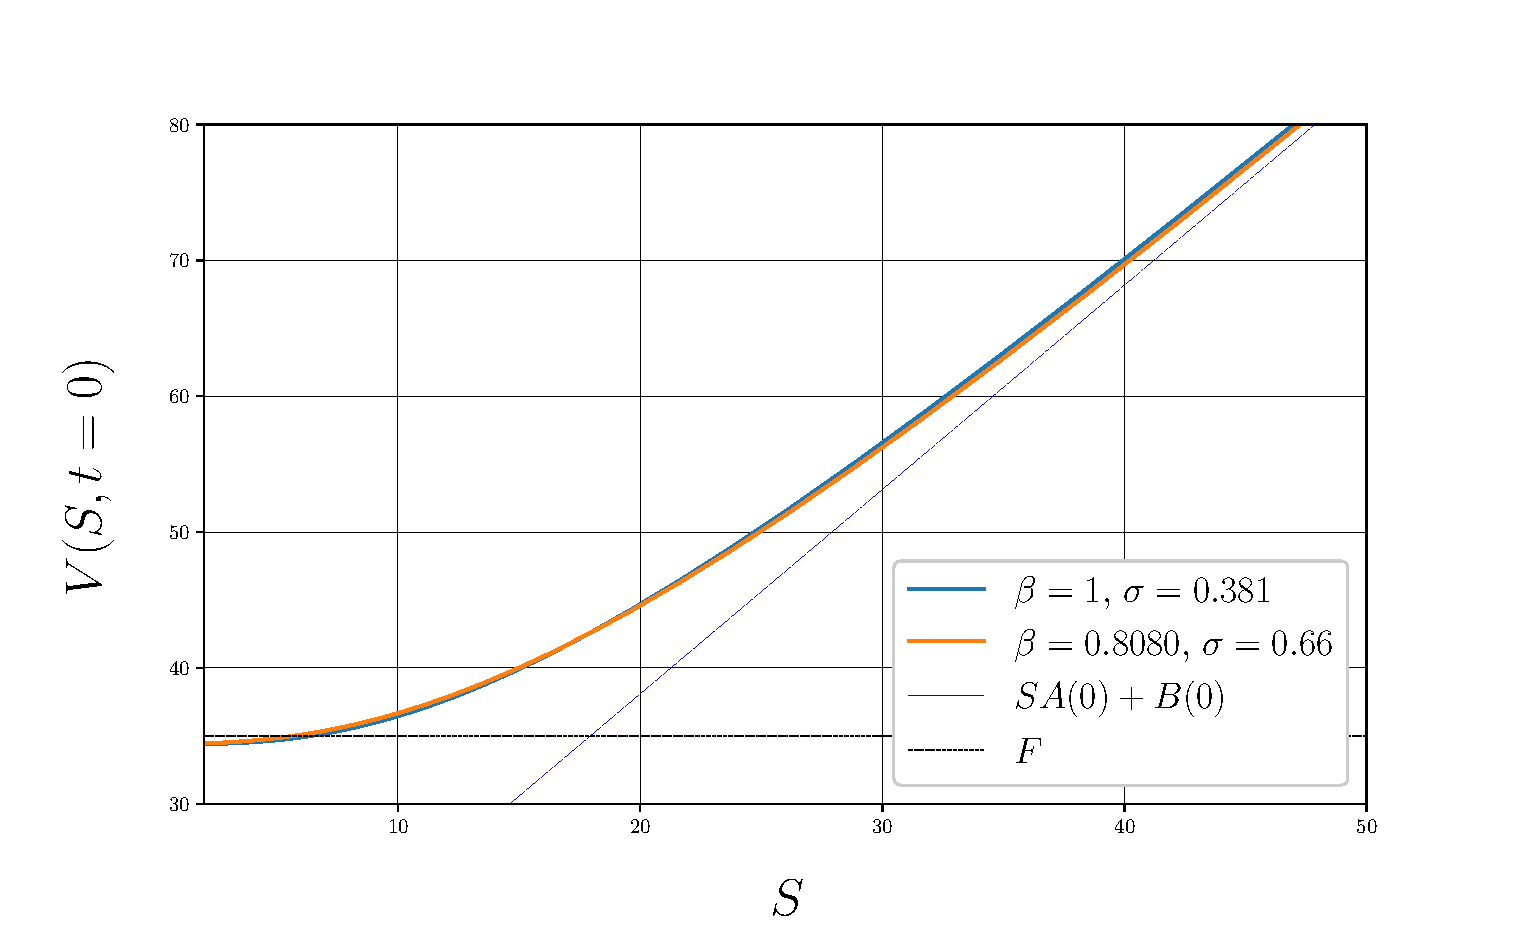
\includegraphics[width=0.45\textwidth]{img/Q1/ComparisonGivenBetaAndSigma.eps}
	\captionsetup{width=.5\linewidth}
	\caption{Value of the option for $\beta=1, \sigma=0.381$ and $\beta=0.8080$ and $\sigma=0.66$.}
	\label{givenBetaSigma}
\end{figure}

In particular, we are told to study the option option value when $\beta=1$ and $\sigma = 0.381$ and $\beta=0.808$ and $\sigma=0.66$. As we can see in Figure \ref{givenBetaSigma}, the results are nearly the same. This means that a relatively low $\sigma$ is compensated with a relatively big $\beta$ and viceversa. Moreover, all the solutions will converge to the same line, because  (\ref{boundary_formula}) does not depend on $\beta$ and $\sigma$. Hence, the role of $\beta$ and $\sigma$ is just to determine how fast the solution converges to $SA(0) + B(0)$ for $S>S^*$ and how plattened it is when $S<S^*$.


